\documentclass[border=5pt,convert={outfile=../_static/\jobname.svg}]{standalone}

\usepackage{tikz}

\begin{document}

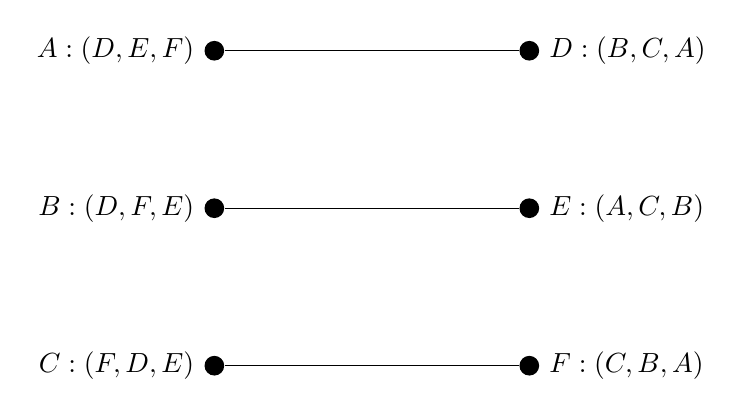
\begin{tikzpicture}

    % Suitors
    \node[fill, shape=circle, inner sep=0, minimum size=0.25cm,
    label=left: {\(A: (D, E, F)\)}] (A) at (0, 0) {};
    \node[fill, shape=circle, inner sep=0, minimum size=0.25cm,
    label=left: {\(B: (D, F, E)\)}] (B) at (0, -2) {};
    \node[fill, shape=circle, inner sep=0, minimum size=0.25cm,
    label=left: {\(C: (F, D, E)\)}] (C) at (0, -4) {};

    % Reviewers
    \node[fill, shape=circle, inner sep=0, minimum size=0.25cm,
    label=right: {\(D: (B, C, A)\)}] (D) at (4, 0) {};
    \node[fill, shape=circle, inner sep=0, minimum size=0.25cm,
    label=right: {\(E: (A, C, B)\)}] (E) at (4, -2) {};
    \node[fill, shape=circle, inner sep=0, minimum size=0.25cm,
    label=right: {\(F: (C, B, A)\)}] (F) at (4, -4) {};

    % Lines
    \draw (A) -- (D);
    \draw (B) -- (E);
    \draw (C) -- (F);

\end{tikzpicture}

\end{document}
